\documentclass[a4paper, 10pt, twoside, notitlepage]{article}
% idioma
\usepackage[spanish]{babel}
\usepackage[utf8x]{inputenc}
\usepackage{graphicx}
\usepackage{multirow} % para las tablas

% graficos
%\usepackage[pdftex]{graphicx}
%\usepackage{wrapfig}

\usepackage{listings}
\lstset{language=C,basicstyle=\small,tabsize=3}

%\usepackage{epic,eepic}
% estilo
\usepackage[footnotesize]{caption}
\usepackage[outer=2cm,inner=4cm,top=2cm,bottom=2cm]{geometry}
\usepackage{fancyhdr}
\usepackage{lipsum}
\usepackage{pdfpages}

\usepackage{color,hyperref}
\definecolor{black}{rgb}{0.0,0.0,0.0}
\definecolor{darkblue}{rgb}{0.0,0.0,0.3}

\hypersetup{colorlinks,breaklinks,
            linkcolor=black,urlcolor=darkblue,
            anchorcolor=darkblue,citecolor=darkblue}

% matematica
\usepackage{amsmath} \usepackage{amsfonts} \usepackage{amssymb}

\title{\textbf{Trabajo Práctico 2:\\Memorias caché} \\}

\author{ \\
         Ronnie Del Pino Cárdenas, \textit{Padrón 93575} \\
          \texttt{ delpinor@gmail.com }       \\
          @delpinor \\
		  [2.5ex]
         Emiliano Vega, \textit{Padrón 76676}     \\
          \texttt{emiliano.vega@mail.com}   \\
          @emiliano.vega   \\                 \\ 
		  [2.5ex]
	 Romina Casal, \textit{Padrón 86429} \\
          \texttt{casal.romina@gmail.com} \\
          @romina
                               \\ 
		  [2.5ex]
		 \\
         \normalsize{2do. Cuatrimestre de 2019}            \\
         \normalsize{86.37 / 66.20 Organización de Computadoras $-$ Práctica Jueves} \\
         \normalsize{Facultad de Ingeniería, Universidad de Buenos Aires} 
       }

\date{}

\begin{document}

\maketitle
% \thispagestyle{empty}   % quita el número en la primer página

% \newpage
% Es un breve resumen de lo que vamos a leer con mayor profundidad en las secciones posteriores, tiene que resaltar lo más importante.
\begin{abstract}
Por medio del presente trabajo práctico se implementó una simulación de una memoria caché de características específicas para analizar su comportamiento con ciertos programas de prueba para medir su performance.

\end{abstract}

% \tableofcontents
% 
% \newpage
% 

\pagestyle{fancy}
\fancyhead{}
\fancyfoot{}
\renewcommand{\sectionmark}[1]{\markright{\thesection\ #1}}
\renewcommand{\headrulewidth}{0.4pt}
%\renewcommand{\footrulewidth}{0.4pt}
\fancyhead[LE]{\nouppercase \rightmark}
\fancyhead[RE, LO]{\bf \thepage}
\fancyhead[RO]{\nouppercase \rightmark}
\fancyfoot[C]{ }
\maketitle
%genera el indice - compilar dos veces
\setcounter{page}{1}
% \tableofcontents
% \newpage

\parskip 7.2pt
%Distinto al resumen, se dice cual es el objetivo principal y se hace un resumen de cada parte que aparece a continuación. 
\section{Introducción}
Usando el programa implementado, se realizará la interpretación de varios programas que ejecutarán comandos definidos para este trabajo simulando accesos a la memoria para analizar el uso de la memoria caché simulada y observar su desempeño.\\

%Una de las secciones más importantes del informe. Aquí se explaya todo lo realizado, problemas encontrados y soluciones propuestas con variantes y métricas.


\section{Proceso de Compilación}
Para la compilación del programa se definió un makefile que ejecuta gcc con opciones convencionales sobre el fuente \textbf{main.c}\\

Creamos un archivo script pruebas.sh que escribirá los resultados en un archivo de salida \textbf{test\_result.txt} \\

\section{Desarrollo}
\normalsize

Para la realización del trabajo práctico se solicitó simular un espacio de memoria principal  de 64KB (array \textbf{mem}) y un caché de 16KB en 8 vias y bloques de 64 bytes (array \textbf{cache}).
Al ser un espacio pequeño de memoria se ha definido ambas estructuras como un array estático.
\textbf{cache} además de su espacio de memoria guarda metadatos de control. Por cada conjunto guarda cuál es el próximo conjunto a reemplazar por política FIFO, y por cada vía guarda también un flag de valid, dirty, el tag de la dirección del bloque, y la propia dirección del bloque en la ram, además de un bloque de 64 bytes para los datos. Si bien el array \textbf{cache} se ha definido como una estructura de words (int) para convivir en la misma los metadatos y el espacio de memoria, se ha controlado que se esté accediendo a nivel byte en las funciones de acceso a memoria implementadas. Para el tipo de simulación que se desea evaluar no impacta en los resultados ya que no estamos midiendo tiempo sino tasa de éxito del caché.

Para la realización de las pruebas se ha solicitado implementar las siguientes funciones en un programa en lenguaje C:

\begin{itemize}
\item[] \textbf{void init()}: Usamos memset() para inicializar a 0 los espacios de memoria que simulan la principal y la caché.
\item[] \textbf{unsigned int get\_offset (unsigned int address)}: devuelve el resto entre la dirección indicada y el blocksize como offset del bloque.
\item[] \textbf{unsigned int find\_set(unsigned int address)}: busca el conjunto de acuerdo a la dirección de memoria solicitada.
\item[] \textbf{unsigned int select\_oldest(unsigned int setnum)}: obtiene cuál será el próximo bloque a reemplazar de ese conjunto.
\item[] \textbf{void read\_tocache(unsigned int blocknum, unsigned int way, unsigned int set)} : transfiere un bloque de memoria RAM al caché
\item[] \textbf{void write\_tomem(unsigned int address, unsigned char)} : transfiere un bloque de memoria caché a la memoria RAM
\item[] \textbf{unsigned char read\_byte(unsigned int address)} : realiza el proceso de acceso a un dato en memoria buscando previamente si existe el dato en el caché y si no existe guarda el bloque en el caché.
\item[] \textbf{void write\_byte(unsigned int address, unsigned char value)} : si encuentra el bloque en el caché, guarda el valor en el caché. Si no lo encuentra, guarda el valor en memoria y caché.
\item[] \textbf{float get\_miss\_rate()} : calcula la cantidad de misses realizados durante la ejecución del programa.
\end{itemize}

\section{Resultados obtenidos}
Ejecutamos el script \textbf{pruebas.sh} y arrojó los siguientes resultados que exporta al archivo \textbf{test\_result.txt}:

\scriptsize
\begin{verbatim}
Pruebas TP2
prueba1.mem
Resultado: 255 
Resultado: 48 
Resultado: 96 
Resultado: 192 
Resultado: 84 
Resultado: 68 
Resultado: 88 
Resultado: 80 
Resultado: 255 
MR: 55.56% 

prueba2.mem
Resultado: 0 
Resultado: 0 
Resultado: 10 
Resultado: 20 
MR: 33.33% 

prueba3.mem
Resultado: 255 
Resultado: 2 
Resultado: 3 
Resultado: 4 
Resultado: 5 
Resultado: 0 
Resultado: 0 
Resultado: 255 
Resultado: 2 
Resultado: 3 
Resultado: 4 
Resultado: 5 
MR: 17.65% 

prueba3b.mem
Resultado: 0 
Resultado: 0 
Resultado: 0 
Resultado: 0 
Resultado: 0 
Resultado: 0 
Resultado: 0 
Resultado: 0 
Resultado: 1 
Resultado: 2 
Resultado: 3 
Resultado: 4 
MR: 62.50% 

prueba4.mem
Resultado: 0 
Resultado: 0 
Resultado: 0 
Resultado: 0 
Resultado: 0 
Resultado: 0 
Resultado: 0 
Resultado: 0 
Resultado: 1 
Resultado: 2 
Resultado: 3 
Resultado: 4 
MR: 62.50% 

prueba5.mem
Dirección no válida: 131072
Resultado: 0 
Dirección o valores no válidos: W 16384,  256
 
Resultado: 0 
Resultado: 0 
Resultado: 0 
Resultado: 0 
MR: 60.00% 
\end{verbatim}

\normalsize



En el programa prueba1.mem observamos que casi todos los misses ocurridos son compulsivos, ya que como partimos de una caché inicializada, los bloques accedidos en la primera parte del programa aún no se encontraban en la caché y están accediendo a distintos conjuntos de la misma, separados por bloques mayores a 64 bytes.\\
En el programa prueba2.mem la tasa de misses es también dada por misses compulsivos(2 misses en total) pero al acceder a menos direcciones que ya se encuentran en caché con más frecuencia, la tasa de fallos resultó menor.
En el programa prueba3.mem ocurre algo similar a prueba2.mem, con la diferencia de que no se trata de las mismas direcciones de memoria, pero sí están en el mismo bloque ya cargado en el caché, es decir se acceden a posiciones contiguas de memoria del primer bloque cargado. Para el caso 3b, si bien se accedes a posiciones contiguas de memoria, los datos no están en el mismo bloque por lo que se produces fallos en mayor número. Prueba4, Idem 3b.
En el programa prueba5.mem tenemos dos comandos que no se pueden procesar. En el primer caso la dirección de memoria es mayor a la máxima(65535) y en el segundo caso se intenta escribir el valor 256 que es mayor a 8 bits(1 byte).


\newpage
\section{Código fuente}
\normalsize
\textbf{Repositorio:github.com/romicasal/orga6620/tree/tp1\_delpinor/tp2}
\subsection{pruebas.sh}
\begin{lstlisting}
echo "Pruebas TP2" > test_result.txt
echo "prueba1.mem" >> test_result.txt
./tp2 prueba1.mem >> test_result.txt
echo "" >> test_result.txt
echo "prueba2.mem" >> test_result.txt
./tp2 prueba2.mem >> test_result.txt
echo "" >> test_result.txt
echo "prueba3.mem" >> test_result.txt
./tp2 prueba3.mem >> test_result.txt
echo "" >> test_result.txt
echo "prueba4.mem" >> test_result.txt
./tp2 prueba4.mem >> test_result.txt
echo "" >> test_result.txt
echo "prueba5.mem" >> test_result.txt
./tp2 prueba5.mem >> test_result.txt

\end{lstlisting}
\subsection{main.c}
\begin{lstlisting}
/*
 * FILAS:
 * Cantidad de conjuntos = Bloques de cache / vias
 * Cantidad de conjuntos = 256 / 8 = 32
 * COLUMNAS:
 * FIFO = 1
 * Valid = 8x1
 * Dirty bit = 8x1
 * TAG =  8x1
 * Nro. de Block = 8x1
 * Datos = 64 * 8 = 512
 * Total = 1 + 8 + 8 + 8 + 8 + 512 = 545
 * |F|...|V|D|T|B|DA|...
 * |1|...|1|1|1|1|64|... |1|1|1|1|64|....
 *  */

#include <stdio.h>
#include <stdlib.h>
#include <math.h>
#include <string.h>
#include <stdbool.h>

#define CONJUNTOS 32
#define FIFOINDEX 0
#define VALIDDIRTYTAG 4
#define ANCHO 545
#define BLOCKSIZE 64
#define MMSIZE 65536
#define OFFSET 6
#define VIAS 8
#define SET 5
#define TAG 5
#define BITS 16
#define FILENAME "prueba3b.mem"
float missRate = 0;
int accesosMemoria = 0;
float misses = 0;
float hits = 0;
unsigned int cache[CONJUNTOS][ANCHO];
unsigned int ram[MMSIZE];

void init();
unsigned int get_offset(unsigned int address);
unsigned int get_tag(unsigned int address);
unsigned int find_set(unsigned int address);
unsigned int select_oldest(unsigned int setnum);
void read_tocache(unsigned int blocknum, unsigned int way, unsigned int set);
unsigned int find_blockIndex(unsigned int way);
void write_tomem(unsigned int blocknum, unsigned int way, unsigned int set);
unsigned char read_byte(unsigned int address);
void write_byte(unsigned int address, unsigned char value);
float get_miss_rate();
unsigned int block_address(unsigned int address);
int main(void) {

    char *line_buf = NULL;
    char bloque1[7];
    char bloque2[7];
    size_t line_buf_size = 0;
    int line_count = 0;
    ssize_t line_size;

    if (!(argc > 1)) {
      fprintf(stderr, "Program filename argument missing\n");
      return EXIT_FAILURE;
    }

    FILE *fp = fopen(argv[1], "r");
    if (!fp) {
        fprintf(stderr, "Error opening file '%s'\n", argv[1]);
        return EXIT_FAILURE;
    }

    line_size = getline(&line_buf, &line_buf_size, fp);

    init();

    while (line_size >= 0) {
        line_count++;
        switch(line_buf[0]) {
        case 'F':
            //printf("FLUSH \n");
            init();
            break;
        case 'W':
            memcpy(bloque1,&line_buf[2], 7);
            int w;
            sscanf(bloque1, "%d", &w);

            char* token;
            char* rest = line_buf;
            int contar = 0;
            while ((token = strtok_r(rest, ",", &rest))) {
                if(contar == 1) {
                    memcpy(bloque2,token, 7);
                }
                contar++;
            }
            int v;
            sscanf(bloque2, "%d", &v );
            if(w >= MMSIZE || v > 255)
                printf("Direccion o valores no validos: W %s \n", bloque1);
            else
                write_byte(w,v);
            break;
        case 'R':
            memcpy(bloque1,&line_buf[2], 7);
            int r;
            sscanf(bloque1, "%d", &r);

            if(r > MMSIZE)
                printf("Direccion no valida: %d\n", r);
            else
                printf("Resultado: %d \n",read_byte(r));
            break;
        case 'M':
            printf("MR: %0.2f%% \n", get_miss_rate()*100);
            break;
        default:
            break;
        }


        line_size = getline(&line_buf, &line_buf_size, fp);
    }

    free(line_buf);
    line_buf = NULL;

    fclose(fp);

    return 0;
}
void init() {
    memset(ram, 0, sizeof(ram));
    memset(cache, 0, sizeof(cache[0][0]) * CONJUNTOS * ANCHO);
    missRate = 0;

}
unsigned int get_offset(unsigned int address) {
    return address % BLOCKSIZE;
}
unsigned int block_address(unsigned int address) {
    return address / BLOCKSIZE;
}
unsigned int get_tag(unsigned int address) {
    int bin[BITS] = { 0 };
    for (int i = 15; i >= 0; i--) {
        bin[i] = address % 2;
        address = address / 2;
    }
    int etiqueta = 0;
    for (int j = 0; j < 5; j++) {
        etiqueta = etiqueta + bin[4 - j] * pow(2, j);
    }
    return etiqueta;
}

unsigned int find_set(unsigned int address) {
    return block_address(address) % CONJUNTOS;
}
unsigned int select_oldest(unsigned int setnum) {
    return cache[setnum][FIFOINDEX];
}
void read_tocache(unsigned int blocknum, unsigned int way, unsigned int set) {
    /* llevo el bloque desde RAM hasta cache */
    for (int i = 0; i < BLOCKSIZE; i++) {
        cache[set][find_blockIndex(way) + VALIDDIRTYTAG + i] = ram[blocknum * BLOCKSIZE + i];
    }
    /* Valid = 1 */
    cache[set][find_blockIndex(way)] = 1;

    /* Guardo el # de bloque */
    cache[set][find_blockIndex(way)+3] = BLOCKSIZE*blocknum;
}
void write_tomem(unsigned int blocknum, unsigned int way, unsigned int set) {
    for (int i = 0; i < BLOCKSIZE; i++) {
        ram[blocknum + i] = cache[set][find_blockIndex(way) + VALIDDIRTYTAG + i];
    }

}
unsigned int find_blockIndex(unsigned int way) {
    return 1 + way * (BLOCKSIZE + VALIDDIRTYTAG);
}
unsigned char read_byte(unsigned int address) {
    accesosMemoria++;
    int hit = 0;
    int via = 0;
    int viaOriginal = 0;
    int valid = 0;
    int tag = 0;
    int set = find_set(address);
    while (!hit && via < VIAS) {
        valid = cache[set][find_blockIndex(via)];
        tag = cache[set][find_blockIndex(via) + 2];
        if ((get_tag(address) == tag) && (valid)) {
            hit = 1;
            hits++;
            break;
        }
        via++;

    };
    if (!hit) {
        via = cache[set][0];
        viaOriginal = via;
        /* Si Dirty bit = 1, escribo en memoria */
        if(cache[set][find_blockIndex(via) + 1] == 1) {
            // printf("M Block: %d",cache[set][find_blockIndex(via) + 3]);
            write_tomem(cache[set][find_blockIndex(via) + 3], via, set);
        }


        /* Llevo el bloque a la Cache */
        read_tocache(block_address(address), via, set);
        /* Actualizo TAG */
        cache[set][find_blockIndex(via) + 2] = get_tag(address);

        via++;
        // Si llego al final, empiezo de nuevo
        if (via >= VIAS) {
            via = 0;
        }

        cache[set][0] = via;
        misses++;
        return cache[set][find_blockIndex(viaOriginal) + VALIDDIRTYTAG + get_offset(address)];
    } else {
        return cache[set][find_blockIndex(via) + VALIDDIRTYTAG + get_offset(address)];
    }
}

void write_byte(unsigned int address, unsigned char value) {
    accesosMemoria++;
    int hit = 0;
    int via = 0;
    int valid = 0;
    int tag = 0;
    int set = find_set(address);
    while (!hit && via < VIAS) {
        valid = cache[set][find_blockIndex(via)];
        tag = cache[set][find_blockIndex(via) + 2];
        if ((get_tag(address) == tag) && (valid)) { // Hit?

            /* Dirty bit = 1 */
            cache[set][find_blockIndex(via) + 1] = 1;

            /* Actualizo cache */
            cache[set][find_blockIndex(via) + VALIDDIRTYTAG + get_offset(address)] = value;
            hit = 1;
            hits++;
            break;
        }
        via++;

    }
    if (!hit) {

        via = cache[set][0];
        /* Si Dirty bit = 1, escribo en memoria */
        if(cache[set][find_blockIndex(via) + 1] == 1) {
            write_tomem(cache[set][find_blockIndex(via) + 3], via, set);
        }
        /* Llevo el bloque a la Cache */
        read_tocache(block_address(address), via, set);

        /* Actualizo TAG */
        cache[set][find_blockIndex(via) + 2] = get_tag(address);
        /* Dirty bit = 1 */
        cache[set][find_blockIndex(via) + 1] = 1;

        /* Actualizo cache */
        cache[find_set(address)][find_blockIndex(via) + VALIDDIRTYTAG + get_offset(address)] = value;
        // Recalcular FIFO
        via++;
        // Si llego al final, empiezo de nuevo
        if (via >= VIAS) {
            via = 0;
        }

        cache[set][0] = via;

        misses++;
    }

}
float get_miss_rate() {
    return misses / accesosMemoria;
}
\end{lstlisting}
\section{Conclusión}
Lo que podemos observar es que no todos los programas funcionan en forma eficiente para la misma arquitectura de caché que use nuestro hardware, lo que se desprende de los diferentes resultados obtenidos en la salida de los programas interpretados.
Según los accesos que tenga durante el programa, tener un caché de tantas vías contribuye a reducir la cantidad de misses de conflicto, pero dependerá de cómo se distribuyan los accesos de memoria. \\
En la mayoría de casos en los que se obtuvo una tasa de MR menor es porque se aprovecha el principio de localidad espacial y temporal, es decir, cuando se acceden a posiciones de memoria contiguas o que se hayan accedido antes.
\vspace{.5cm}
%Referencias o recursos utilizados durante la investigación para la resolución del trabajo práctico 
\begin{thebibliography}{5}
 \bibitem{} Hennessy, John L. and Patterson, David A., Computer Architecture: A Quantitative Approach, Third Edition, 2002.
 \bibitem{} Kernighan, Brian, and Ritchie, Dennis, The C Programming Language.
\end{thebibliography}

\clearpage



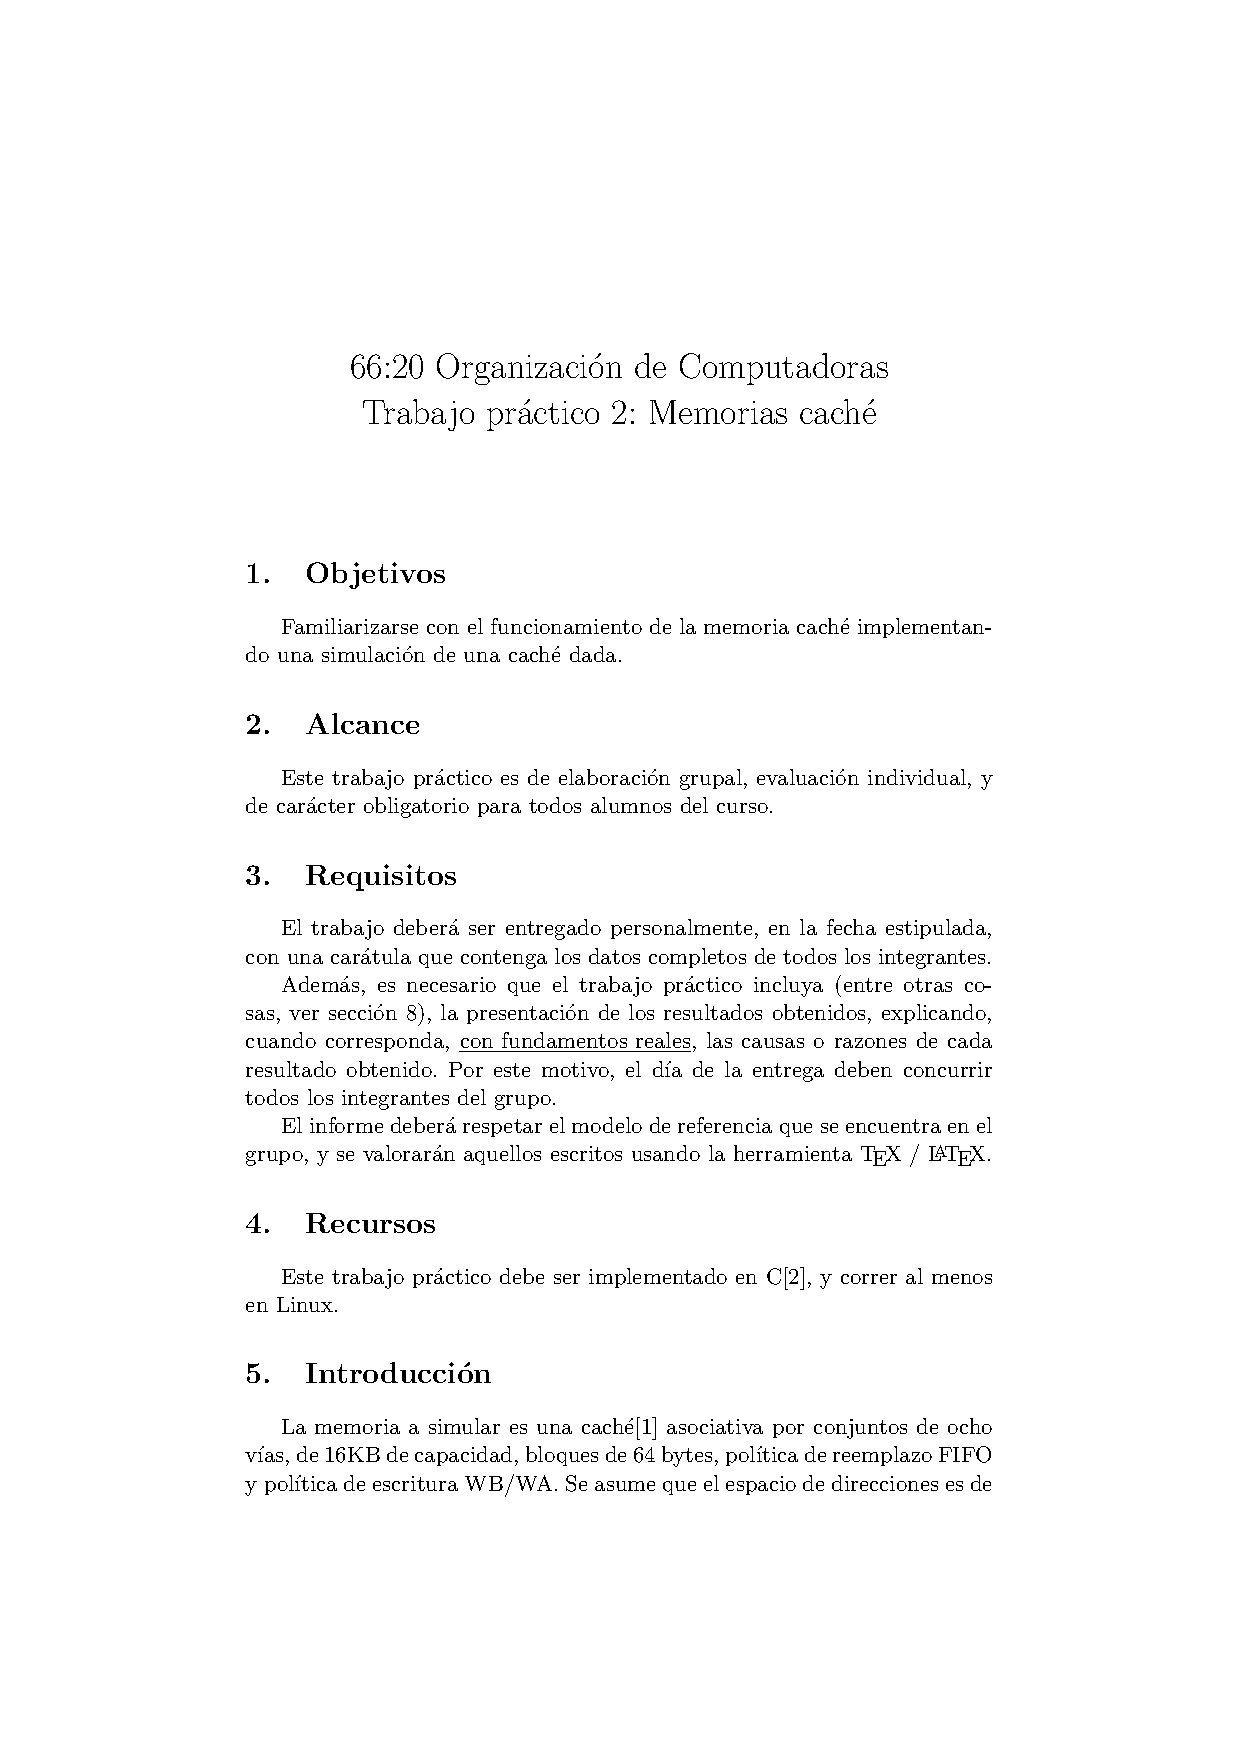
\includepdf[pages={-}]{tp2-q2-2019.pdf}


\end{document}
